\chapter{Model predictive control}
\label{ch:mpc}
In this chapter, the framework conditions of the MPC are described by answering the questions: (i) what is controlled? (ii) How is controlled? (iii) Which curves are controlled? (iii) What data are used? Also, the constraints, the cost function, and the workflow of the MPC script are introduced. The objective of this investigation is to obtain a control signal for the heat pump of the reference building that considers grid services and occupancy comfort. There, the investigation stays in a simulation environment. \newline

\section{Framework conditions of the MPC}
\label{section:FrameworkMPC}
The objective of the MPC is to optimise the control signal of the reference building $\mathbf{u} = (u_1 \enspace u_2)^T = (\dot{Q}_\text{heating} \enspace \dot{Q}_\text{HP})^T$. Thereby, we consider the heat flows of the building in the MPC simulation but, we calculate with a characteristic diagram of the heat pump the electrical control signal $P_\text{HP}$ later. The controlled output is the inside temperature $\mathbf{y} = T_\text{inside}$, which we calculate with the thermal model from \autoref{holeModel}. The desired curves of the $\mathbf{y}$ depend on the presents of occupants, which is determined on an occupancy schedule. Past data of the weather and the dynamic price of the electricity $dP$ \nomenclature[P]{dP}{dynamic Price of the electricity } is used for the simulation environment. 

\subsection{Characteristic diagram of the heat pump}
\label{subsec:charcteristicDiagramHP}
The characteristic diagram of the heat pump is interpolated with the characteristic values specified by the producer \cite{TUM}. We assume an operation at the nominal power of the heat pump. As \autoref{fig:HeatpumpKennfeld} shows, the electrical power $P_\text{HP}$ depends on the outside temperature $T_\text{outside}$ and the required heat flow $\dot{Q}_\text{HP}$. Further, the heat pump can generate negative $\dot{Q}_\text{HP}$ when cooling is desired. The optimisation of the MPC computed the $\dot{Q}_\text{HP}$, and the $T_\text{outside}$ is known at every time step, then the characteristics of the heat pump are used to calculate the $P_\text{HP}$. The optimised control signal as heat flows cannot directly influence the grid. Therefore, $P_\text{HP}$ is needed to analyse the effects on the grid. Furthermore, converting $\mathbf{u}$ into $P_\text{HP}$ simplifies the analysis, as we then only consider positive values.
    \begin{figure}[h]
            \centering
            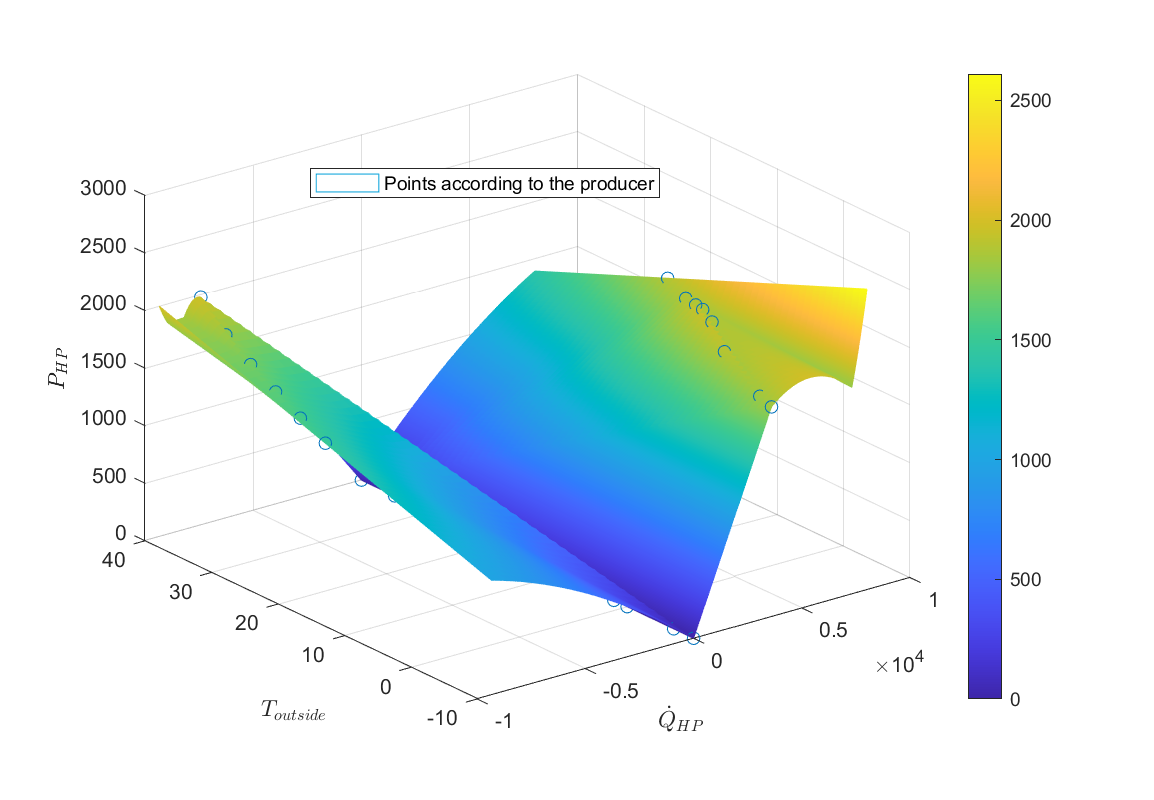
\includegraphics[width=8cm,height=6.5cm]{figure/HeatPumpV55nenn.eps}
           \caption{Interpolation of the characteristic diagram of the heat pump with nominal power according to \cite{TUM}}
           \label{fig:HeatpumpKennfeld}
    \end{figure}
    
\subsection{Occupancy schedule}
\label{subsec:OccupancySchedule}
The \autoref{fig:OccupancySchedule} presents the occupancy schedule. It summarises the working time of occupants with a green bar. We assume that persons are in the reference building from Monday to Thursday from 6 am to 7 pm and on Friday from 6 to 6 pm. The assumption is made according to experience values and means that there is a high probability that persons will be in the building during this time.  
    \begin{figure}[h]
            \centering
            
\includegraphics[width=15cm]{figure/Occupancy schedule.PNG}
           \caption{Occupancy schedule of the reference building}
           \label{fig:OccupancySchedule}
    \end{figure}

\subsection{Past data}
\label{subsec:PastData}
    The data used are from the same period as the training data for the model estimation. As a disturbance variable, we use the recording of diffuse radiation and outside temperature in Energy Lab 2.0. The MPC is simulated over nine days, a little more than a week, to consider the occupancy schedule at least  once.\newline
    The dynamic price of the electricity  $dP$ is made available on the website of the Bundesnetzagentur \cite{Bundesnetzagentur-smard}. Here we use the wholesale prices on the stock exchange as an indicator of grid services. The price is an intersection between supply and demand. Consequently, when the price is low, we can assume an excess of electricity on the grid. It is precisely then that it is particularly suitable to operate our heat pump to obtain electricity from the grid. In the opposite case, the same applies: If the price is high, it is unfavourable to operate the heat pump. At such a time, it is particularly suitable to supply power from the grid. In the opposite case, the same applies: if the price is high, it is unfavourable to operate the heat pump. \newline
    However, negative prices can also arise in retail. Negative prices would undesirably change the costs of the cost function, which will be explained in more detail later at a suitable time. To avoid negative prices, we sum the absolute minimum value of the $dP$ to every value of $dP$. Thus, we shift the curve of $dP$ into positive, as shown in \autoref{fig:Gridverschiebung}. In the later use, we calculate with the dynamic price of electricity $dP$ in the unit of $\frac{\text{\euro}}{Wh}$.
    \begin{figure}[h]
            \centering
            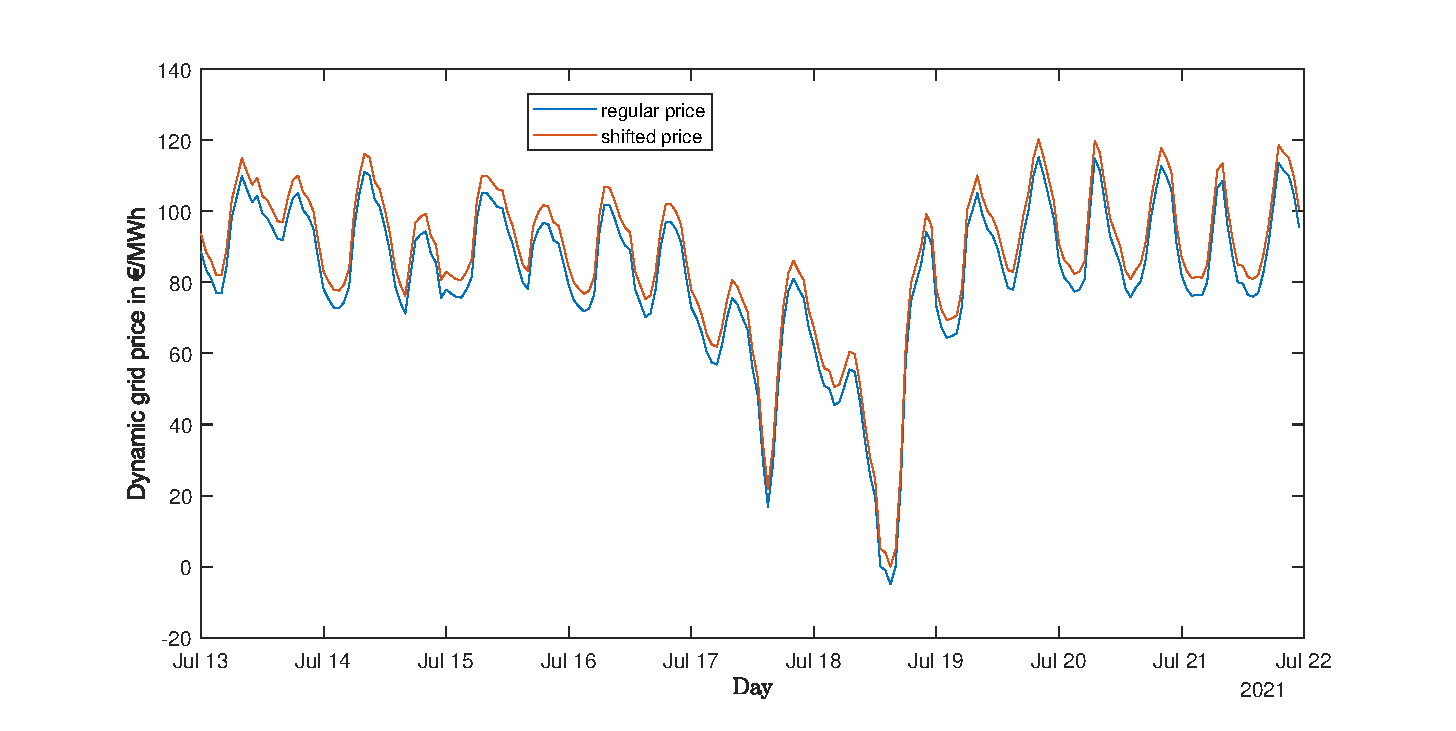
\includegraphics[width=15cm,height=8cm]{figure/Grid_data_Verschiebung.eps}
           \caption{Dynamic price of electricity \cite{Bundesnetzagentur-smard} and shifted dynamic price of electricity}
            \label{fig:Gridverschiebung}
    \end{figure}
    
\section{The Constraints}
\label{section:theconstraints}

The constraints depend on the physical limitations of the installations in the building, such as the heat pump, the underground floor heating, and the water reservoir, or of comfortable reasons. Also, the integration method of the model is included in the constraints. The subsequent section gives an overview of the constraints.

\subsection{Constraints of the control signals}
\label{subsec:COnstraintU}
The producer's specifications restrict $\dot{Q}_\text{HP}$ the maximum and minimum heat flow of the heat pump for nominal power by heating with the inlet temperature of 55°C and by cooling with the inlet temperature of 18°C \cite{TUM}. The maximum $\dot{Q}_\text{heating}$  is limited according to the underground floor heating calculation, where the set power of every room is counted and we sum it for the complete building \cite{Roth_Auslegung.2020}. The computation of the required cooling power predicts 2246 W needed power by 34.5°C outside temperature in July \cite{SEFIngenieurgesellschaftMBH.2019}. To be more flexible with higher outside temperatures, we round the minimum $\dot{Q}_\text{heating}$ to 2300 W.\newline
Further, we define a constraint $u_1 \cdot u_2 \geq 0$ to avoid simultaneous heating of building and cooling of the water reservoir or reversed. That would be energy waste.
The set $\mathbb{U_k}$ summarise mathematically the constraints.
\begin{equation}
    \label{ConstraintU}
    \mathbb{U_k} = \{\mathbf{u_k}| -2300 W \prec \dot{Q}_\text{heating} \prec 5283 W \wedge -9340 W \prec \dot{Q}_\text{HP} \prec 8010 W | u_1 \cdot u_2 \geq 0\} 
\end{equation}

\subsection{Constraint of output}
\label{subsec:constrainY}
The Umweltbundesamt \cite{Umweltbundesamt.7.10.2021} recommends an inside temperature of 18°C for some rooms, such as the kitchen. We expand the recommendation to a minimum $T_\text{inside}$ of 18°C for all rooms. The maximum inside temperature refers to the German technical rules for workplaces \cite{Bund.2021}, wherein a maximum of 26°C as room temperature is prescribed. The slack variable $\eta_\text{k}$ allows a variance of the given temperature range during a penalty in the cost function. Thus, we have a soft constraint, and we can obtain the feasibility of the optimisation problem during a deviation of the temperature range \cite{Drgona.2020}. The constraint is represented in the set $\mathbb{Y_k}$ as follows:  
\begin{equation}
    \label{ConstraintY}
    \mathbb{Y_k} = \{\mathbf{y_k}| 18 \text{°C} - \eta_k \prec T_\text{inside} \prec 26 \text{°C}+ \eta_k\} 
\end{equation}

\subsection{Constraints of the states}
\label{ConstraintX}
The calculation of the water reservoirs maximal inner energy $U_\text{WR}$ is explained in \autoref{waterModel} with \autoref{eq:max.Energie}. The minimum $U_\text{WR}$ lies by 0 J. The set $\mathbb{X}_{5,k}$ describes the constraint for the fifth element of the state vector.
\begin{equation}
    \label{ConstraintX5}
    \mathbb{X}_{5,k} = \{x_\text{5,k}| 0 J \prec U_\text{WR} \prec 96370000 J\} 
\end{equation}
A further constraint, which relates to the states, is the integration method as discussed below.

\subsection{Integration method and its constraint}
\label{COnstaintIntegration}
As an integration method, we use a explicit single-step method,which means that we need the values of the actual time step $k$ to compute the next. Possible methods are the Heun's method, the Euler and the Runge-Kutta method. The decision is made in favor of the Runge-Kutta method because the fourth order makes it more precise than the methods mentioned. The following equation shows the calculation for the next time step using the Runge-Kutta method with the sample time $T_\text{s}$ and the function $f(\mathbf{x_k},t_\text{k},\mathbf{u_k},\mathbf{d_k}) = \mathbf{\dot{x}_\text{k}}$ according the state-space formulation (see \autoref{eq:statespace}) \cite{KaiFurmansMarcusGeimerBalazsPritzCarstenProppe.WS1920}.

    \begin{align}
        \label{Runke-Kutta}
        a_k^{(1)} = T_s \cdot f(\mathbf{x_k},t_\text{k},\mathbf{u_k},\mathbf{d_k}) \\
        a_k^{(2)} = T_s \cdot f(\mathbf{x_k}+\frac{a_k^{(1)}}{2},t_k+\frac{T_s}{2},\mathbf{u_k},\mathbf{d_k})\nonumber\\
        a_k^{(3)} = T_s \cdot f(\mathbf{x_k}+\frac{a_k^{(2)}}{2},t_k+\frac{T_s}{2},\mathbf{u_k},\mathbf{d_k})\nonumber\\
        a_k^{(4)} = T_s \cdot f(\mathbf{x_k}+a_k^{(3)},t_k+T_s,\mathbf{u_k},\mathbf{d_k})\nonumber\\
        \nonumber\\
        \mathbf{x_{k+1}} = \mathbf{x_k} + \frac{1}{6}\cdot (a_k^{(1)} + 2 a_k^{(2)} + 2 a_k^{(3)} + a_k^{(4)})\nonumber
    \end{align}
The constraints accommodate the integration method for calculating the next time step according to the determined thermal model.
Important to note is that the time step of the integration is chosen in accordance with the discretization of the model. The model is estimated with the discrete values of the reference building, where the measuring points are sampled every two minutes. For example, to achieve a $T_\text{s}$ of one hour, the $T_\text{s}$ is described as $30 \cdot 2 min$. The two minutes are already included in the model by estimation. The two minutes are already included in the model due to the estimation. Therefore, we multiply the $\mathbf{\dot{x}_\text{k}}$ by 30 to bring forward a time step of one hour. It is considered that the thermal model is composed of two submodels. The water reservoir sub-model, which is modelled using the white-box approach, requires a different conversion to advance one hour. Here we convert watts to joules per hour. In the MPC, this difference is compensated by a factor directly in the state-space formulation of the model.

\section{The Cost function}
\label{section:thecostfunction}

The cost function penalise the deviation from the desired requirements. On the one hand, we have to guaranty thermal occupant comfort in the building. On the other hand, we prefer to heat with the heat pump during convenient grid service. Both subjects are represented in the cost function below.
    \begin{equation}
        \text{minimize} \sum_{k=1}^{N-1} w_\text{1}\cdot (y_\text{k}-y_\text{track})^2 + w_\textbf{2}\cdot(u_\text{2,k}\cdot dP_\text{k})^2 + w_\text{3} \cdot \eta_\text{k}^2
        \label{eq:costfunctatsächlich}
    \end{equation}
A pleasant air temperature is 22°C for living rooms, working rooms, and the bathroom \cite{Umweltbundesamt.7.10.2021}. As discussed in \autoref{ch:modelling}, we model the reference building as a single-zone building, wherein most rooms are working rooms. We decide to use the median temperature of all rooms of the recommended temperatures for the complete building. Thus, the desired temperature is $y_\text{track} = 22$°C.\newline
The expression $(y_\text{k}-y_\text{track})^2$ represents the comfort requirement in the cost function. The squaring of $(y_\text{k}-y_\text{track})$ avoid a minimising of the cost function due to negative $y_\text{k}$ values. The same proceeding is with the expression of the grid service $(u_\text{2,k}\cdot dP_\text{k})^2$. We exclude negative values of $dP_\text{k}$ (how is explained in \autoref{subsec:PastData}) because we would generate the wrong effect with a negative $dP_\text{k}$. After squaring, the expression would maximise the cost function during a appropriate time for grid services. Without a squaring, we would support energy consumption while its not needed or we would penalise a cooling by we having a negative $u_\text{2,k}$.\newline
We can adjust the preference of the requirements by the weightings $w_\text{1}$ and $w_\text{1}$. How much deviation is allowed from the temperature range in the soft constraint is determined by the weighting $w_\text{3}$.\newline
The size of the cost for the requirements are different. When considering the constraints, $y_\text{k}-y_\text{track}$ can reach a maximum deviation of 4 K (without soft constraint), while $u_\text{2,k}\cdot dP_\text{k}$ is in a lower order of size due to the unit $\frac{\text{\euro}}{Wh}$. To compensate this, a factor is introduced that gives the comfort requirement a weaker weighting in the cost function. The factor is integrated into the weighing $w_\text{1}$ as shown in the following table. In general, we vary the weights $w_\text{1}$ and $w_\text{2}$ of the cost function from $ i= 0$ to 1 in 0.1 steps. As shown in table \autoref{tab:weighting factor}, the comfort with $w_\text{1}$ and the grid service with $w_\text{2}$ are always weighted in opposite directions.\newline
\begin{table}[h]
    \centering
    \begin{tabular}{c|c|c}
         $w_\text{1}$ & $w_\text{2}$ & $w_\text{3}$ \\
        $\frac{1}{4} \cdot i$ & $i=1-j$ & 0.001
    \end{tabular}
    \caption{Weighting factor}
    \label{tab:weighting factor}
\end{table}
Occupant comfort is only necessary if persons are present in the building. Therefore, we consider the cost function during absence without the comfort therm by setting $w_\text{1}$ to zero according to the occupancy schedule, which results in the following simplification of the cost function during absence.
    \begin{equation}
        \text{minimize} \sum_{k=1}^{N-1} w_\textbf{2}\cdot(u_\text{2,k}\cdot dP_\text{k})^2 + w_\text{3} \cdot \eta_\text{k}^2
        \label{eq:costfunctionAbwesenheit}
    \end{equation}
The procedure aims to generate more flexibility for the objective of grid services. This scenario with the changing cost function is the basic scenario for this thesis.  %Weshalb so energie sparen erklären

\section{Workflow of the MPC script}
\label{section:workflowMPC}
The approach in the MPC script is determined by the use of the tool CasAdi. CasADi is an open-source tool for nonlinear optimisation and algorithmic differentiation and is characterised by a symbolic framework. Especially, mixed-integer optimal control problems, such as an MPC, are of particular interest \cite{JoelA.E.Andersson.2018}. We can combine CasAdi with MATLAB through a simple import.\newline
The figure below gives an overview of the workflow of the MPC script. First, we create the parameter, all known sizes, and the optimisation variables symbolically. Then the inequalities of the constraints are set in a loop over the prediction horizon with the symbolic variables. The cost function is also indicated symbolically for the horizon. Afterwards, the initial values for the optimiser are determined. To specify the initial state for the first MPC step, we choose a constant control signal $\mathbf{u_k} = [0\enspace0]^T$, a state $\mathbf{x}$ within the temperature range, and determine with the Runge-Kutta method the curve over the horizon. A half charged water reservoir is a further assumption for the initial state. We pass the values of the initial state of the optimisation variations and the parameters to the solver. Then, the optimisation problem is solved with the Ipopt (\textbf{I}nterior \textbf{P}oint \textbf{Opt}imiser) solver, which is appropriate for large and sparse nonlinear programming \cite{JoelA.E.Andersson.2018}. As a result, we obtain the optimised $\mathbf{u_k}$ over the horizon. Now, after each time step, a new initial state is calculated with the curves of the states and the output from the new disturbance variables and the optimum $\mathbf{u_k}$ over the horizon.
    \begin{figure}[h]
            \centering
            \def\svgwidth{0.75\textwidth}
            \input{figure/workflowMPC2.pdf_tex}
            \caption{Workflow of the MPC script}
            \label{fig:workflowMPC}
    \end{figure}
    
\section{Choice of weightings and horizon}
\label{Choise of weigtings and horizon}
In the following, we analyse the horizon length $N$ \nomenclature[P]{N}{ length of the predictive horizon} and the effects of the weightings on the requirement of occupancy comfort and grid services for the basic scenario. For a better comparison we define an average comfort AC \nomenclature[A]{AC}{Average Comfort}, which is a size of the average deviation of the $y$ from the $y_\text{track}$ over the simulation time only during presence of occupants, expressed by $y_\text{k,occ} - y_track$. The calculation of AC is described in the following equation with the number of time steps with occupants $n_\text{occ}$.
\begin{equation}
    \label{eq:average comfort}
    AC = \frac{\sum_{k,occ}^{n_\text{occ}} |y_\text{k,occ} - y_\text{track}|}{n_\text{occ}}
\end{equation}
On the other hand, we define the costs for grid services GS \nomenclature[A]{GS}{Costs for grid services} over the whole simulation time (with the number of time steps $n$) as the sum of the electrical power of the heat pump $P{HP,k}$ multiplied with the dynamic price of electricity $dP_\text{k}$:
\begin{equation}
    GS = \sum_{k}^n P_{HP,k}\cdot dP_\text{k}
\end{equation}
In theoretical considerations, we should obtain a higher level of AC with less weighting of comfort and a higher level of GS with less weighting of grid services. Furthermore, a larger or shorter horizon $N$ differs in computation time and finding the optimal solution. While a longer N requires more computation time and may not find a solution, a shorter $N$ may not find the optimal solution. Due to finding the optimal solution a larger horizon should result in less costs for the requirements. In general, the horizon should depict the dynamics of the controlled system. \newline
The theoretical considerations are inspected in the subsequent sections for the basic scenario over the simulation time of nine days.   

\subsection{Average comfort and grid services over the weightings}
\label{subsec:Average comfort and grid services over the weightings}
The following figure presents the behaviour of the AC and GS for the different weightings $w_\text{1}$ and $w_\text{2}$ with $N = 24h$. We compare the behaviour also for different horizon $N$ to verify the feasibility and the expected behaviour. The corresponding figures are showed in \autoref{sec:Average comfort and grid services} and the values of AC and GS for different horizons exposed in the following tables.\newline
We notice a monotone behaviour of the average comfort and the grid services according to their weightings and feasible solutions. The less costs with increasing horizon length is only for the average comfort notable, expecting the case $w_\text{1}=0$. In this case, we consider not the comfort in the cost function. Therefore, the values of AC are coincidental, also relating to the horizon length.\newline
An explanation for higher cost in GS with longer horizon is that the thermal reaction of the building is known over a longer time and the control signal reacts early for a better adaption of the comfort.
    \begin{figure}[h]
            \centering
            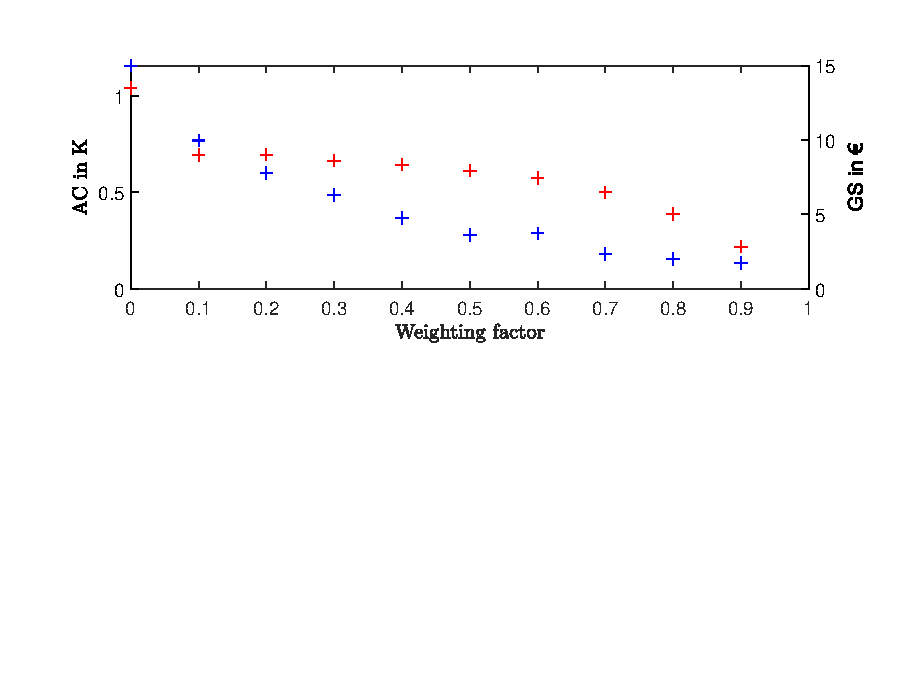
\includegraphics[width=15cm,height=8cm]{figure/AC_und_GS_24h.eps}
           \caption{AC and GS for N = 24h}
            \label{fig:AC_und_GS_24h}
    \end{figure}
    
    \begin{table}[h]
    \centering
    \begin{tabular}{c|c|c|c|c|c|c|c|c|c|c|c}
         weighting factor i&0&0.1&0.2&0.3&0.4&0.5&0.6&0.7&0.8&0.9&1  \\
         \hline
         AC by N = 12 h&\\
         AC by N = 18 h&\\
         AC by N = 24 h&\\
         AC by N = 30 h&\\
    \end{tabular}
    \caption{AC for different N}
    \label{tab:AC for different N}
    \end{table}
    
    \begin{table}[h]
    \centering
    \begin{tabular}{c|c|c|c|c|c|c|c|c|c|c|c}
         weighting factor i&0&0.1&0.2&0.3&0.4&0.5&0.6&0.7&0.8&0.9&1  \\
         \hline
         GS by N = 12 h&\\
         GS by N = 18 h&\\
         GS by N = 24 h&\\
         GS by N = 30 h&\\
    \end{tabular}
    \caption{GS for different N}
    \label{tab:GS for different N}
\end{table}
    

     
    
\subsection{Choice of the horizon}
\label{subsec:ChoiceHorizon}